\documentclass[letterpaper,twocolumn,10pt]{article}
\usepackage{usenix}

\usepackage{booktabs}
\usepackage{graphicx}
\usepackage{subcaption}
\usepackage{amsmath}
\usepackage{amsfonts}
\usepackage{enumitem}
\usepackage{multirow}
\usepackage{lineno}
\usepackage{listings}
\usepackage{courier}
\usepackage{xcolor}
\usepackage{url}
\usepackage{comment}
\usepackage{hyperref}

\newcommand{\colorcomment}[2]{\textcolor{#1}{#2}}
\newcommand{\taggedcolorcomment}[3]{\colorcomment{#1}{\textbf{#2} #3}}
\newcommand{\todo}[1]{\colorcomment{red}{\textbf{TODO:} #1}}
\newcommand{\refs}{\colorcomment{red}{\textbf{REFS}}}
\newcommand{\reza}[1]{\taggedcolorcomment{blue}{RC:}{#1}}
\newcommand{\tapan}[1]{\taggedcolorcomment{orange}{TB:}{#1}}
\newcommand{\yossi}[1]{\taggedcolorcomment{red}{YO:}{#1}}

\newcommand{\tbd}[1]{\textcolor{red}{#1}}


\definecolor{lstbg}{RGB}{245,247,250}
\definecolor{lstkw}{RGB}{0,70,160}
\definecolor{lstcm}{RGB}{110,110,110}
\lstdefinelanguage{page}{morekeywords={div,iframe,backdrop-filter,position},
  sensitive=true, morecomment=[s]{<!--}{-->}, morecomment=[s]{/*}{*/}}
\lstset{language=page, basicstyle=\ttfamily\fontsize{7}{8.2}\selectfont,
  keywordstyle=\color{lstkw}\bfseries, commentstyle=\color{lstcm}\itshape,
  backgroundcolor=\color{lstbg}, frame=single, rulecolor=\color{black!20}, framesep=3pt,
  columns=fullflexible, keepspaces=true, aboveskip=6pt, belowskip=0pt,
  xleftmargin=4pt, xrightmargin=4pt, showstringspaces=false}

\makeatletter
% The usenix style reserves a 2.5in box for the title block; shrink it.
\def\@maketitle{\newpage
 \begin{center}%
  \vspace*{-0.3in}%
  {\Large\bf \@title \par}%
  \vskip 0.15in
  {\large\it \lineskip .5em
   \begin{tabular}[t]{c}\@author\end{tabular}\par}%
 \end{center}%
 \vskip 0.1in}
% Tighter paragraph headings and float spacing.
\renewcommand\paragraph{\@startsection{paragraph}{4}{\z@}{4pt plus 1pt minus 1pt}{-0.6em}%
  {\normalfont\normalsize\bfseries}}
\setlength{\textfloatsep}{8pt plus 2pt minus 2pt}
\setlength{\floatsep}{6pt plus 2pt minus 2pt}
\makeatother

\title{WIP: Behind the Backdrop: Pixel Stealing Through the GPU Cache}
\author{}
\date{}

\microtypecontext{spacing=nonfrench}
\begin{document}
\maketitle

\section{Introduction}

The security of the modern web relies critically on the rigorous enforcement of the Same-Origin
Policy (SOP). \emph{Pixel stealing} is a class of cross-origin attacks in which an attacker infers the visual content of a rendered element displayed in a cross-origin iframe, thereby undermining SOP's confidentiality goals. The attacker cannot read the embedded pixels directly. Instead, it magnifies one (or more) pixels at a time, covers it with an SVG filter whose amount of work depends on the pixel's color, and measures a side effect of that work. Repeating this for every pixel rebuilds the image, which may show a username or other private text.

Early pixel-stealing research ~\cite{Stone2013PixelPerfectTiming} exploited
data-dependent branches in browser SVG filter implementations. As browser vendors moved toward
constant-time implementations, researchers sought new surfaces. Pixel Thief~\cite{pixelthiefsec24} exploits content-dependent memory accesses in the CPU implementation of SVG filters, but requires forcing Chrome into a non-default CPU rendering mode. EXAM~\cite{xu2025exam} leverages the system-level cache shared between the CPU and the GPU on Apple M-series SoCs, which is not generalizable to all hardware. Hot Pixels~\cite{taneja2023hotPixels} and Hertzbleed~\cite{Hertzbleedsp23} rely on pixel-dependent power and frequency behavior. GPU.zip~\cite{gpuzip} exploits graphical data compression,
observed through DRAM traffic and the CPU cache. To protect against these attacks, Chrome~151 (July 2026) stopped the application of SVG filters to cross-origin iframes altogether~\cite{chromestatus}, removing the critical step that all filter-based attacks rely on.

In this work in progress, we show that Chrome's mitigation can be bypassed, and we build a
pixel-stealing attack that differs from prior work in three respects. (i)~By placing an empty
element over the iframe and giving it a CSS \texttt{backdrop-filter}, our attack page applies the filter to the iframe's pixels in Chrome despite the mitigation. (ii)~Our attack relies mostly on contention in the GPU cache, which we measure with a WebGPU compute kernel. (iii)~We decide each pixel's color with a trained machine-learning model rather than a threshold, aiming for improved robustness in environments where noise can disrupt simple thresholding logic. We confirm with hardware counters that the attack contends on the GPU cache, and show that it recovers images accurately, at a speed comparable to prior work, and under CPU-side defensive noise.

Our choice of the GPU cache is motivated by the hypothesis that the GPU cache hierarchy itself
constitutes an under-mitigated and widely available leakage surface in browsers. Browsers use the GPU to draw SVG filters by default, and every GPU has its own caches. We show that when a filter does more work, it pushes more data through the GPU cache, and any other program running on the GPU at the same time slows down because the two compete for the same cache. The GPU cache is an attractive place to measure this effect: it is separate from the CPU cache, so CPU-side noise reaches it less, plus it is small and used by few processes, so the filter's activity stands out against little background noise. We stress that pixel values leak can across multiple vectors. In our work, we demonstrate that the GPU cache is one of them.


%==============================================================================
\section{Experiments and Contributions}

\paragraph{Experimental setup.} We ran our experiments in Google Chrome on a Lenovo ThinkPad P14s laptop with an NVIDIA T550 GPU, running Windows~11, and on a Google Pixel~6a
phone with an Arm Mali-G78 GPU, running Android~17. The victim page, loaded from a different
origin, shows a black-and-white checkerboard image.

\paragraph{Bypassing Chrome's mitigation.} To steal a pixel, the attack page embeds the victim page in an iframe and magnifies it so that one pixel fills a fixed area. Prior attacks then placed the SVG filter on a \emph{parent} of the iframe. Chrome draws the parent together with everything inside it, including the iframe's pixels, and runs the filter on the result. Chrome's mitigation blocks this~\cite{chromestatus}. Chrome tracks the visual effects applied to
the page in an \emph{effect tree} that mirrors the nesting of page elements. When it draws an
iframe, it now walks up this tree, and if any ancestor of the iframe carries an SVG filter, it skips that filter.

The check, however, only looks at the iframe's ancestors. Our attack instead places the filter on an empty element that is a \emph{sibling} of the iframe's container, positioned exactly on top of the magnified pixel (Listing~\ref{lst:page}), and applies it as a \texttt{backdrop-filter}. Unlike a regular filter, which processes an element's own content, a backdrop filter processes whatever is drawn \emph{behind} the element. Chrome therefore draws the iframe first, takes a snapshot of the pixels behind the empty element, and runs the filter on that snapshot. In the snapshot, the cross-origin pixel is just an ordinary pixel, and because the filter is not on any ancestor of the iframe, Chrome's check never triggers. The filter thus processes the cross-origin pixel again.

\begin{lstlisting}[caption={Page structure of the attack page to bypass chrome's mitigation},label={lst:page},captionpos=b,float=t]
<div class="clip">
  <div class="zoom">                <!-- one pixel -->
        <iframe src="https://victim.example"></iframe>
    </div>
</div>
<div class="filter-layer"></div>      <!-- on top -->

.clip, .filter-layer { position: absolute; top: 0; left: 0;}
.filter-layer { backdrop-filter: url(#filter); }
\end{lstlisting}

\paragraph{Measuring the filter through the GPU cache.} We use the same filter as
GPU.zip~\cite{gpuzip}. The filter creates random noise and multiplies it with the pixel, again and again, in a chain of 20 layers. Over a white pixel every layer produces an image of noise; over a black pixel every layer produces an all-black image. A white pixel therefore makes the GPU move much more data through its cache. To keep the filter running, we give the noise a new random seed in every frame, which forces Chrome to redraw the filter each time. To measure the filter's activity, we adapt the cache-occupancy approach~\cite{shusterman2019robust} to the GPU. The WebGPU API that lets a web page run programs, called \emph{compute kernels}, on the GPU. Our attack kernel repetitively sums the elements of a buffer about the size of the GPU cache, and the attack page times each run of the kernel. When the filter pushes the kernel's data out of the GPU cache, the kernel has to fetch it again from memory and takes longer. Figure~\ref{fig:traces} shows this effect: the kernel runs slower while the filter processes a white pixel than a black one.

\begin{figure}[t]
  \centering
  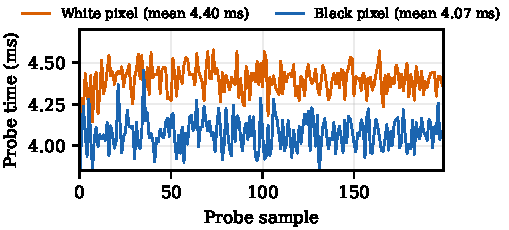
\includegraphics[width=\columnwidth]{figures/traces.pdf}
  \caption{Kernel execution time while the filter processes a white or a black pixel.}
  \label{fig:traces}
\end{figure}

\paragraph{Stealing an image.} The attack steals one pixel at a time. For each pixel, it runs the kernel a fixed number of times, for example 100, and records how long each run takes. We call each measured run time a \emph{sample} and the samples collected for one pixel a \emph{trace}. A single sample is too noisy to reveal the pixel's color, but a whole trace is not. We classify each trace as white or black with a convolutional neural network (CNN), which the attacker trains beforehand on traces collected over pixels whose color it already knows. The number of samples per pixel trades speed for accuracy. (Table~\ref{tab:speed}).

\begin{table}[t]
\centering\small
\setlength{\tabcolsep}{3pt}
\begin{tabular}{llrr}
\toprule
Attack & Hardware & Pixels/s & Accuracy \\
\midrule
GPU.zip~\cite{gpuzip} & AMD Vega 8 & 6.20 & 93.4\% \\
GPU.zip~\cite{gpuzip} & Intel UHD 770 & 2.70 & 96.2\% \\
GPU.zip~\cite{gpuzip} & Intel UHD 630 & 2.00 & 99.6\% \\
Pixnapping~\cite{pixnapping} & Galaxy S25 & 2.11 & 95.1\% \\
Hertzbleed~\cite{Hertzbleedsp23} & Intel i7-8700 & 1.16 & 99.4\% \\
Sched.\ Disclosure~\cite{scheduleddisclosure} & Intel Meteor Lake & 0.14 & 96.3\% \\
\midrule
Ours & NVIDIA T550 & 2.00 & 98.4\% \\
Ours & Pixel 6a & \tbd{--} & \tbd{--} \\
\bottomrule
\end{tabular}
\caption{Speed and accuracy of pixel-stealing attacks that utilize the GPU.} \tapan{Mobile to be filled}
\label{tab:speed}
\end{table}

\paragraph{Root cause of the attack.} If the attack works as we claim, the filter should interfere with the kernel inside the GPU's memory hierarchy, and more so over a white pixel than over a black one. We verify this with NVIDIA's profiler, Nsight Compute, which reads the GPU's hardware counters. Since the profiler only supports CUDA programs, we rewrote our kernel in CUDA and ran it while Chrome applied the filter over a white pixel, over a black pixel, or not at all.
Table~\ref{tab:l2} shows two effects. First, as GPU.zip~\cite{gpuzip} observed, the filter
generates more memory traffic over a white pixel: the kernel reads 125.7\% more data from the
GPU's memory (DRAM) than over a black one. We note that the filter also contends with the kernel in the GPU's L2 cache. With no filter running, 82\% of the kernel's
accesses hit in the cache; with the filter, the hit rate drops to 51\% over a black pixel and to
38\% over a white one. Over a white pixel the kernel has 14.8\% fewer cache hits and 34.7\% more
cache misses than over a black one. The timing difference therefore stems from both DRAM traffic
and GPU cache contention, and both arise inside the GPU. We
also recorded the GPU's clock frequency during the attack. It differed by only 1.6\% between white and black pixels, so on this GPU the timing difference does stem primarily from frequency changes.

\begin{table}[t]
\centering
\small
\setlength{\tabcolsep}{4pt}
\begin{tabular}{l r@{\hspace{2pt}}c@{\hspace{2pt}}l r@{\hspace{2pt}}c@{\hspace{2pt}}l r@{\hspace{2pt}}c@{\hspace{2pt}}l}
\toprule
Filter over & \multicolumn{3}{c}{L2 hits} & \multicolumn{3}{c}{L2 misses} & \multicolumn{3}{c}{DRAM read (KB)} \\
\midrule
Nothing         & 18,432 & $\pm$ & 0     & 4,096  & $\pm$ & 0     & 170   & $\pm$ & 51 \\
Black           & 15,138 & $\pm$ & 3,192 & 15,343 & $\pm$ & 6,274 & 740   & $\pm$ & 501 \\
White           & 12,899 & $\pm$ & 2,818 & 20,659 & $\pm$ & 2,629 & 1,670 & $\pm$ & 1,457 \\
\midrule
White vs.\ black & \multicolumn{3}{c}{$-$14.8\%} & \multicolumn{3}{c}{+34.7\%} & \multicolumn{3}{c}{+125.7\%} \\
\bottomrule
\end{tabular}
\caption{L2 cache hits and misses and DRAM reads of the kernel while Chrome applies the filter (NVIDIA T550, mean $\pm$ std).}
\label{tab:l2}
\end{table}

\paragraph{Robustness to CPU-side defensive noise.} Finally, we tested whether noise-injection
defenses designed for CPU cache attacks stop our attack. We ran a CPU-side defense that injects
noise into the CPU cache from the browser~\cite{flipstress} and let the attacker train and attack under this noise. GPU.zip, whose signal is read through the CPU, recovers the image with only X\% accuracy, while our attack reaches 74\% (Table~\ref{tab:noise}). Three properties explain the difference. First, the GPU cache is separate from the CPU cache, so CPU-side noise does not reach it. Second, the GPU cache is small and shared by few processes, so the filter's activity occupies a large part of it against little background noise. Third, a trained classifier can learn what the noisy timings look like, whereas a fixed threshold is easily shifted by noise. \tapan{Not writtten well}

\begin{table}[h!]
\centering\small
\begin{tabular}{lc}
\toprule
Attack & Accuracy under CPU-side defensive noise \\
\midrule
GPU.zip~\cite{gpuzip} & X\% \\
Ours & X\% \\
\bottomrule
\end{tabular}
\caption{Image recovery accuracy under CPU-side defensive noise.} \tapan{To be Filled}
\label{tab:noise}
\end{table}

{\footnotesize
\bibliographystyle{plain}
\bibliography{references}
}

\end{document}
